\documentclass[border=10pt]{standalone}
\usepackage{tikz}
\usetikzlibrary{arrows.meta, positioning, shapes.geometric, calc}

\begin{document}
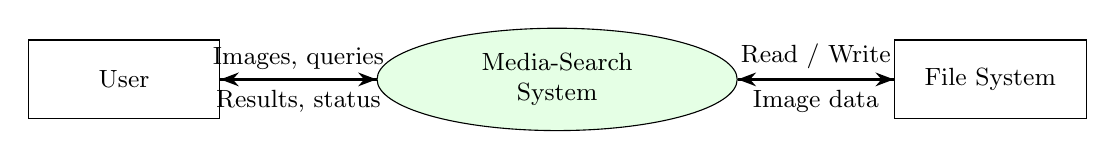
\begin{tikzpicture}[
  ext/.style ={draw, rectangle, text width=2.2cm, minimum height=1.0cm,
               align=center, font=\small},
  proc/.style={draw, ellipse, text width=3.0cm, minimum height=1.3cm,
               align=center, font=\small, fill=green!10},
  arr/.style ={->, >=Stealth, thick},
]
\node[ext]  (user) at (0,0)   {User};
\node[proc] (sys)  at (5.5,0) {Media-Search System};
\node[ext]  (fs)   at (11,0)  {File System};

\draw[arr] (user.east) -- node[above, font=\small]{Images, queries} (sys.west);
\draw[arr] (sys.west)  -- node[below, font=\small]{Results, status} (user.east);
\draw[arr] (sys.east)  -- node[above, font=\small]{Read / Write} (fs.west);
\draw[arr] (fs.west)   -- node[below, font=\small]{Image data} (sys.east);
\end{tikzpicture}
\end{document}
